% !TEX root = BLDC_Schrittmotoren_Technologie.tex
\renewcommand{\autoren}{Severin Schendel	}
\newpage
\section{Vergleich der Antriebsarten}
\subsection{Bürstenloser Gleichstrommotor}
	
\begin{quote}
"Bürstenlose Gleichstrommotoren, kurz BLDC („Brushless DC-Motoren), sind -  entgegen ihrer Bezeichnung - Drehstrom-Synchronmaschinen: Der Läufer folgt einem magnetischen Drehfeld, die Bewegung ist synchron zur Wechselspannung, die an die Wicklungen angelegt wird. Dieser Motortyp wird häufig als „Bürstenloser Gleichstrommotor“ bezeichnet, da er in vielen Applikationen bürstenbehaftete Gleichstrommotoren („brushed DC“, Kommutatormotoren) ersetzt. Bei einem bürstenbehafteten Gleichstrommotor wird eine Gleichspannung angelegt, die durch einen mechanischen Wechselrichter im Motor - die Bürsten - einen drehzahlunabhängigen Wechselstrom erzeugt.

Zusammen mit einer elektronischen Ansteuerung, die die Funktion der Bürsten übernimmt und aus den eingespeisten Gleichstrom in Wechselstrom umwandelt, entspricht der BLDC-Motor im Verhalten einem bürstenbehafteten Gleichstrommotor ohne die in der Lebensdauer begrenzten Bürsten.  BLDC-Motoren werden deshalb auch als EC („electronically commutated“)-Motoren bezeichnet, um sie von mechanisch kommutierten bürstenbehafteten Motoren abzugrenzen."
\end{quote}
(Quelle: \cite{BLDCNanotec})
\begin{figure}[h]  % [h] bedeutet, dass das Bild genau an dieser Stelle im Text erscheint
\centering\includegraphics[width=0.8\textwidth]{images/BLDC_Prinzipschaltung}
\caption{BLDC Prinzipschaltung, V1-V6 MOSFETS \newline (Quelle: \cite{PrinzipBLDC})}
\label{PrinzipBLDC}
\end{figure}

\subsection{Schrittmotoren}

\begin{quote}
"Für das Verständnis der Funktionsweise eines einfachen Schrittmotors ist es hilfreich, die enge Verbindung zu seinem Vorläufer, dem bürstenlosen Gleichstrommotor (BLDC-Motor), zu verstehen. BLDC-Motoren sind rotorseitig mit Permanentmagneten ausgestattet. Die Magneten richten den Rotor zu am Umfang des Stators angeordneten Elektromagneten aus, wenn diese mit Strom versorgt werden. Der Rotor kann dann bewegt werden, indem der Stromfluss durch die Elektromagnete umgekehrt wird oder einige der Elektromagnete ein- und ausgeschaltet werden. Der Rotor dreht sich, wenn die Stromumkehrung oder die Schaltsequenz rotatorisch abläuft. Die Geschwindigkeit der Drehbewegung kann durch Ändern der Schaltfrequenz erhöht oder verringert werden.

Diese Beziehung zwischen den stationären Elektromagneten des Ständers und den Permanentmagneten des Rotors stellt auch das Grundprinzip für den Permanentmagnet-Schrittmotor dar. Neben dieser Grundversion des Schrittmotors gibt es weitere Ausführungen. Bei einer dieser Ausführungen, dem Hybridmotor, werden die Eigenschaften von Reluktanz- und Permanentmagnet-Schrittmotor kombiniert. Der Hauptunterschied zwischen dem Schrittmotor und dem BLDC-Motor besteht darin, dass die Permanentmagneten (Pole) im Rotor auf eine Anzahl zwischen 12 und 200 (Auflösung $30^\circ$ bzw. $1,8^\circ$) erhöht werden. Je mehr Pole ein Schrittmotor hat, desto besser ist seine Auflösung um die Drehachse, allerdings kosten mehr Pole nicht nur mehr Geld, sondern auch Drehmoment.

Obwohl BLDC- und Schrittmotoren auf demselben grundlegenden Funktionsprinzip beruhen, sind Schrittmotoren für gewöhnlich sehr viel komplexer. Die zusätzlichen Pole des Schrittmotors bedeuten, dass der Rotor in vorhersagbaren Stufen schrittweise verfahren werden kann. Der Schrittmotor kann seine Drehstellung auch halten, solange die Elektromagnete eingeschaltet sind. Während sich der BLDC-Motor besser für durchgängige Drehbewegungen eignet, kann der Schrittmotor richtig glänzen, wenn es darum geht, zu einem präzisen Winkel zu drehen oder eine genaue Position zu halten. Der Schrittmotor ist sehr viel flexibler in der Änderung der Drehbewegung. Er kann schnell zu einem spezifischen Winkelwert drehen, anhalten, weiterdrehen oder bei Bedarf sogar die Drehrichtung ändern."
\end{quote}
(Quelle: \cite{BLDCNanotec})


\subsection{Möglichkeiten der Kommutierung}
